\documentclass[11pt]{article}

\usepackage{amsmath}
\usepackage{amssymb}
\usepackage{enumitem}
 \usepackage{graphicx}
\usepackage[margin=1in]{geometry}

\begin{document}

\title{Graph-Augmented Digital Twins for Political Organizations: Experiment Proposal}
\maketitle

\section{Introduction}

Political parties play a central role in representative democracies by aggregating the preferences of members, supporters, and elected officials into collective positions that guide legislative and governmental action. This process requires reconciling diverse and evolving viewpoints across multiple policy domains.

In practice, parties rely on a limited set of mechanisms to infer and synthesize internal preferences, such as surveys, conventions, and roll-call votes. While these instruments provide structured information, they are costly to deploy, tend to overrepresent the most politically active members, and capture only partial and infrequent snapshots of a broader distribution of opinions. As a result, the translation of dispersed political signals into coherent collective positions remains constrained.

Recent advances in artificial intelligence have expanded the set of tools available to process and synthesize complex information. Among these, Large Language Models (LLMs) have demonstrated the ability to generate coherent text by integrating information from diverse and distributed sources, enabling new forms of large-scale text analysis and synthesis.

In the context of political representation, these developments open the possibility of constructing computational pipelines that operate over structured political information. In this study, we construct structured representations of political actors using knowledge graphs derived from speeches, voting records, and position papers. These representations encode relationships between actors, policy issues, and expressed positions in a formal and queryable format.

On top of these representations, we deploy agents to simulate how different political actors might respond to new policy questions. The outputs of these agents are then combined through an aggregation procedure to produce consensus statements for a given political party and policy issue.

This setup raises a natural empirical question: when individuals compare these machine-generated consensus statements to those produced by political parties (e.g., position papers or press releases), which do they perceive as closer to their own views? In other words, can the computational aggregation of distributed political signals produce collective statements that align more closely with the individuals they are intended to represent?

Our study evaluates these perceptions by focusing on individual-level alignment between participants’ own positions and different types of textual summaries across multiple policy contexts.

In this document, we provide a detailed description of the experiment. Specifically, we (i) describe the data sources and computational procedures used to generate the texts presented to participants; (ii) outline the design of the online experiment; and (iii) discuss implementation details, including sampling, questionnaire structure, and data collection procedures.


\section{Consensus Statements Design}

\begin{figure}[htbp]
\centering
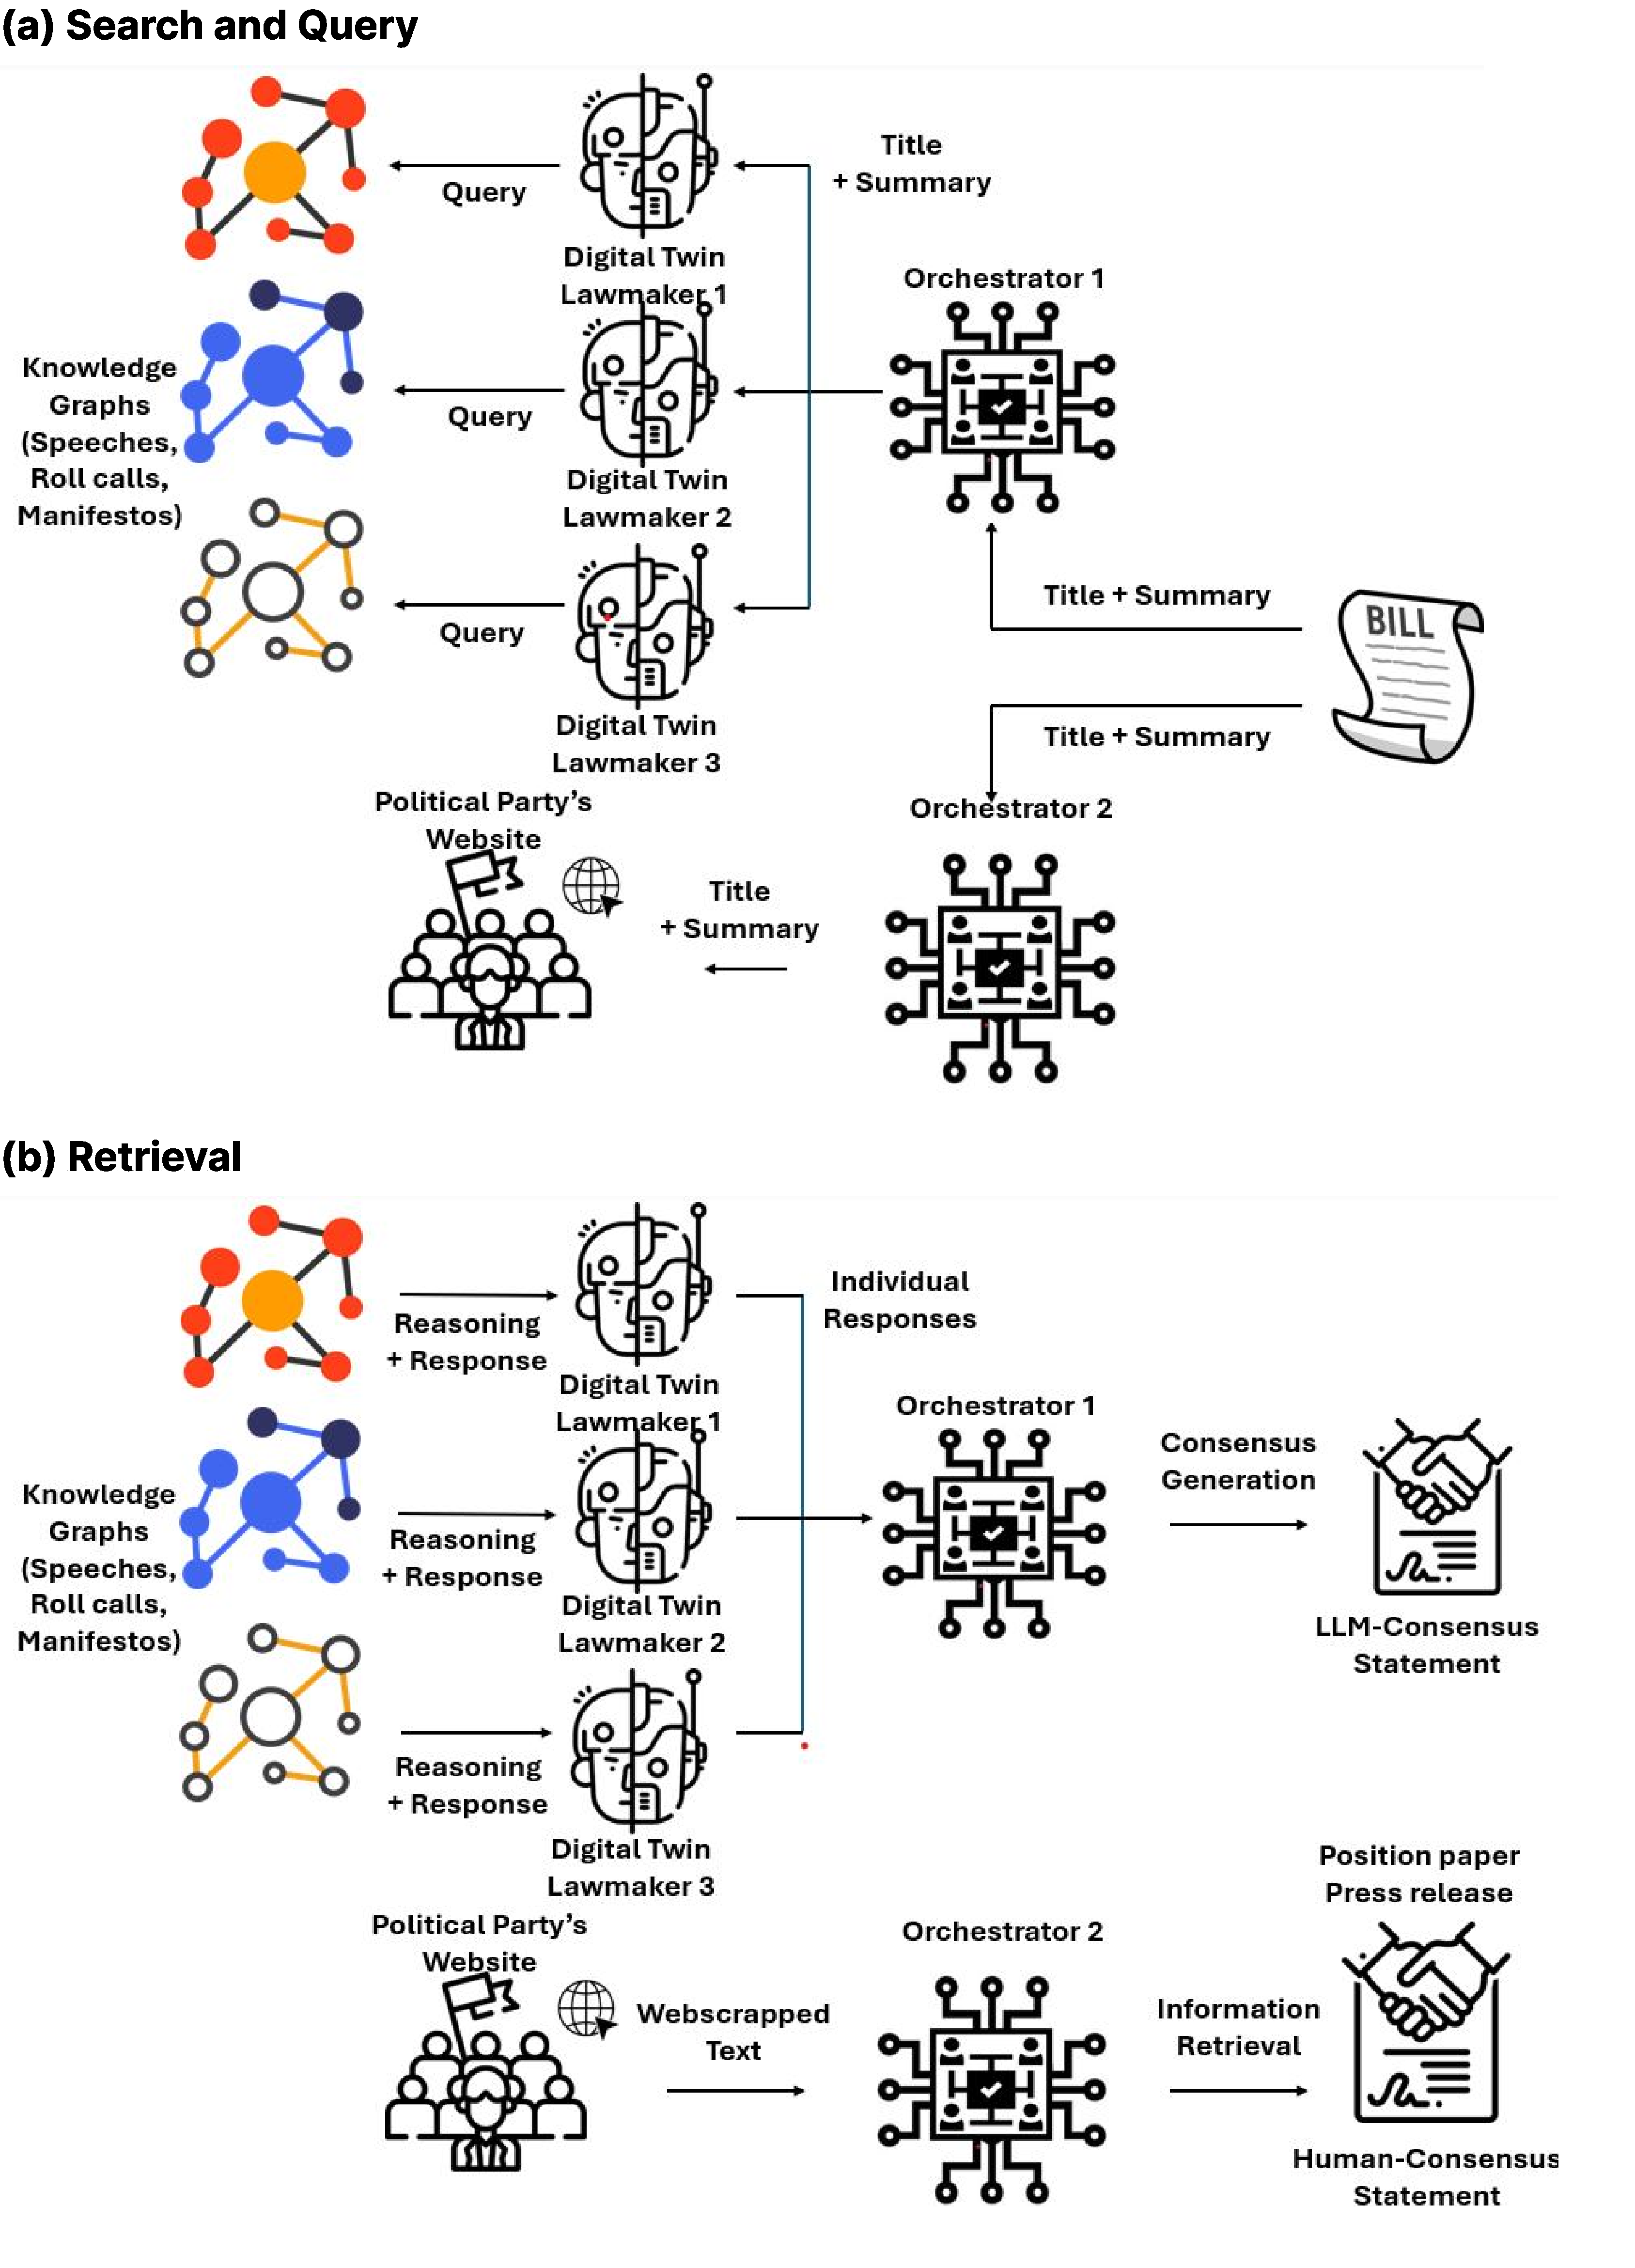
\includegraphics[width=\linewidth, height=0.85\textheight, keepaspectratio]{figures/Synthesis.pdf}
\caption{Computational pipeline for consensus statement generation. 
Panel~(a): Orchestrator~1 dispatches each bill's title and summary to 
the digital twin lawmakers, who query their individual knowledge graphs 
(speeches, roll-call votes, manifestos) to retrieve relevant prior 
positions; Orchestrator~2 simultaneously queries the political party's 
website. Panel~(b): each digital twin returns a reasoning chain and 
response to Orchestrator~1, which aggregates them into an LLM-consensus 
statement; in parallel, Orchestrator~2 applies information retrieval 
over web-scraped party communications to retrieve position papers and press releases.}
\label{fig:consensusstatements}
\end{figure}

This section describes the computational pipeline used to generate the two types of consensus statements presented to participants: \textit{LLM-consensus statements}, produced by aggregating the outputs of simulated political agents, and \textit{human-consensus statements}, retrieved from official party communications. The pipeline is illustrated in Figure~\ref{fig:consensusstatements}.

\subsection{Data Sources}

We collect data from the Swiss parliament and official websites of political parties to build computational representations and generate the different texts presented to participants.


\subsection{Knowledge Graph Construction}

Our pipeline is grounded in three primary sources of structured political information. For each Swiss lawmaker included in the study, we collect (i) parliamentary speeches, (ii) roll-call voting records, and (iii) party manifestos, newsletters and journals. These documents are processed and encoded as \textit{knowledge graphs}, in which nodes represent political actors, policy issues, and expressed positions, and edges capture the relationships between them. This structured representation makes the information formally queryable and allows downstream agents to retrieve relevant context in a targeted and reproducible manner.


\subsection{Agent Architecture}

The generation of LLM-consensus statements relies on a multi-agent architecture composed of two layers: \textit{digital twin lawmakers} and \textit{orchestrators}. The architecture operates in two sequential stages, depicted respectively in panels (a) and (b) of Figure~\ref{fig:consensusstatements}.

\paragraph{Digital Twin Lawmakers.} For each legislator in the sample, we instantiate a dedicated LLM agent — a digital twin — whose behavior is conditioned on that individual's knowledge graph. As shown in panel (a) of Figure~\ref{fig:consensusstatements}, when a policy question is introduced, each orchestrator first transmits the bill's title and summary to the digital twin lawmakers under its supervision. Each digital twin then queries its associated knowledge graph to retrieve relevant prior positions, votes, and speeches, and generates an individual response that reflects the simulated lawmaker's reasoning and stance. This response, together with its supporting reasoning chain, is returned to the orchestrator, as illustrated in panel (b).

\paragraph{Orchestrators.} Two orchestrators coordinate the pipeline.

Orchestrator 1 manages the digital twin lawmakers: it receives the bill's title and summary as input, dispatches this information to each agent, collects their individual responses, and runs a \textit{consensus generation} procedure over these outputs to produce a single synthesized statement (upper path of panel (b) in Figure~\ref{fig:consensusstatements}). This LLM-consensus statement represents the aggregated position of the simulated legislative group on the given policy issue.

Orchestrator 2 operates in parallel on party-level data. It receives the same bill title and summary and applies an \textit{information retrieval} procedure to extract the position papers and press releases concerning the same bill (lower path of panel (b) in Figure~\ref{fig:consensusstatements}). The output of this procedure constitutes the human-consensus statement — a summary grounded in official party communications authored by human actors.

\subsection{Pipeline Summary}

The full pipeline produces, for each bill and each party, two textual summaries that are structurally comparable but procedurally distinct. As Figure~\ref{fig:consensusstatements} makes clear, the LLM-consensus statement is constructed bottom-up, by simulating and aggregating the individual positions of lawmakers as encoded in their knowledge graphs. The human-consensus statement is constructed top-down, by retrieving the official positions published by the political party. Both types of statements are generated without exposing participants to their provenance, enabling a clean comparison of perceived alignment in the experiment described in the following section.

\section{Human Validation Design}

Our experiment examines whether individuals affiliated with a political party perceive their own viewpoints as more accurately reflected in LLM-consensus statements — generated by aggregating the outputs of digital twin lawmakers — than in human-consensus statements produced by official political parties, such as position papers and press releases.


More concretely, each participant completes the following procedure for 20 distinct bills:
\begin{enumerate}

\item Participants indicate their preferred political party and (optionally) report some sociodemographic characteristics along with questions about their opinion about artificial intelligence and technology in general. All data are collected anonymously, with no personally identifying information retained at any stage of the procedure, in accordance with applicable research ethics standards.

\item Participants are presented with a concise summary of a bill that was subject to a Swiss referendum from 2024 onward.

\item Participants report their own position and arguments on the bill.

\item Participants are shown three consensus statements in randomized order and asked to select the one that best represents their own viewpoint on the issue. The three statements are: (i) a human-consensus statement, retrieved by Orchestrator 2 from the official position papers or press releases of the participant's preferred political party; (ii) an LLM-consensus statement generated by Orchestrator 1 through the consensus generation procedure applied to the individual responses of digital twin lawmakers; and (iii) an LLM-consensus statement produced by an equivalent pipeline in which the digital twin lawmakers are instantiated from a non-fine-tuned LLM, without access to lawmaker-specific knowledge graphs.

\item Participants provide a brief justification for their choice.

\end{enumerate}


\section{Evaluation}

\subsection{Evaluation Dimensions}

Participants evaluate the three consensus statements along the following 
dimensions. For each question, participants select one of the three 
statements presented to them.

\paragraph{Representativeness and preference.}
\begin{enumerate}[label=\roman*.]
    \item Which of the three statements best reflects your own position 
    on this issue?
    \item Which of the three statements would you most want your 
    political party to adopt as its official stance?
    \item Which of the three statements do you find most credible 
    and trustworthy?
\end{enumerate}

\paragraph{Pluralism and balance of perspectives.}
\begin{enumerate}[label=\roman*., resume]
    \item Which of the three statements best reflects how complex you 
    personally find this issue?
    \item Which of the three statements felt most like it was trying 
    to persuade you, rather than inform you?
\end{enumerate}

\paragraph{Language and accessibility.}
\begin{enumerate}[label=\roman*., resume]
    \item Which of the three statements is written in language that 
    feels most familiar and natural to you?
    \item Which of the three statements was easiest to understand?
\end{enumerate}

\paragraph{Values and personal arguments.}
\begin{enumerate}[label=\roman*., resume]
    \item Which of the three statements best captures the values and 
    concerns that matter most to you regarding this issue?
    \item Which of the three statements would you be most comfortable 
    sharing with someone to explain your position on this bill?
\end{enumerate}

\paragraph{Decision support.}
\begin{enumerate}[label=\roman*., resume]
    \item If you were undecided on this bill, which of the three 
    statements would be most helpful in guiding your decision?
\end{enumerate}

\subsection{Evaluation Framework}

For each evaluation dimension, we compute the share of participants who 
selected each type of consensus statement.

To examine how these choice proportions vary across participant 
characteristics, we estimate random forest models in which the outcome is 
the chosen statement type and the predictors are socio-demographic variables 
--- including age, gender, education, political orientation, and preferred 
political party. We also conduct two-sample $t$-tests to assess whether 
choice proportions differ significantly across demographic subgroups.

\section{Sample Size Determination}

\begin{figure}[htbp]
\centering

\includegraphics[width=\linewidth, height=0.85\textheight, keepaspectratio]{DigiRep/figures/sample_size_sigma.pdf}
\caption{Required sample size for estimating the proportion of participants who perceive the LLM-generated consensus as representative of their own position, plotted against outcome variability $\sigma$ for different margins of error $E$ (95\% confidence level).}
\label{fig:samplesize}
\end{figure}

The minimum number of participants required for this experiment is determined using the standard formula for proportion estimation in an infinite population:
\begin{equation}
n = \left( \frac{Z_\alpha \, \sigma}{E} \right)^2,
\end{equation}
where $Z_\alpha$ is the critical value of the standard normal distribution associated with the chosen confidence level, $\sigma$ captures the expected variability in the binary outcome of interest, that is, whether a participant perceives the LLM-generated consensus statement as representative of their own position, and $E$ is the margin of error, expressing the maximum tolerable deviation between the estimated proportion and the true population value. Smaller values of $E$ demand proportionally larger samples.

Here we use a 95\% confidence level and thereby $Z_\alpha = 1.96$, which means that across repeated replications of the experiment, 95\% of the resulting intervals would bracket the true population proportion. Assuming relatively homogeneous responses, we set $\sigma = 0.05$. Finally, assuming a very small value ($\E = 0.005$), this gives $n = (0.98/0.05)^2 \approx 384$. A sample of $n = 384$ is therefore adopted as the minimum required number of participants.

Figure~\ref{fig:samplesize} plots the minimum number of participants as a function of $\sigma$, with several lines representing different values of $E$.

\section{Bills Content}

All bills presented to participants are drawn from Swiss popular initiatives and referendums held between 2024 and 2026. For each bill, the full texts are retrieved directly from the published records of the Swiss Parliament's website. These full texts are then processed using GPT-5-nano to produce a detailed and accessible description of the bill, including its specific practical implications, which is what participants are ultimately presented with as the basis for their evaluation.

Twenty bills are considered in this experiment:

\subsection*{Cash, public media, and climate}

\paragraph{``Cash is freedom'' initiative (popular initiative, 8 March 2026)}
Popular initiative to anchor in the Constitution that the Swiss franc remains the national currency and that cash (banknotes and coins) must continue to exist and be widely available, limiting the risk of a fully digital cashless economy.

\paragraph{Counter-proposal to the cash initiative (federal counter-proposal, 8 March 2026)}
Parliamentary constitutional proposal that also guarantees cash and the Swiss franc, but with more flexible wording that leaves greater room for the development of digital payments and future monetary policy.

\paragraph{SRG Initiative -- ``200 francs are enough!'' (popular initiative, 8 March 2026)}
Initiative seeking to reduce the mandatory household levy that finances the public broadcaster (SRG SSR) to 200 Swiss francs per household and to exempt companies entirely, thereby substantially cutting the resources of public service media.

\paragraph{Climate Fund Initiative (popular initiative, 8 March 2026)}
Initiative to create a constitutionally anchored climate fund dedicated to large-scale financing of renewable energy and other measures against global warming, ensuring additional and stable resources for the ecological transition.

\subsection*{Taxation, population, and neutrality}

\paragraph{Individual taxation (Federal Act on Individual Taxation, approved 8 March 2026)}
Reform that replaces joint taxation of married couples with individual taxation of each adult, aiming to remove the ``marriage penalty'' and make the tax system more neutral with respect to family status and female labour-market participation.

\paragraph{``No to ten-million Switzerland'' initiative (popular initiative, vote on 14 June 2026)}
Initiative of the Swiss People’s Party (SVP) to set a constitutional ceiling of 10 million inhabitants and oblige the federal government to curb immigration once the population reaches 9.5 million, including the option of terminating the free movement agreement with the EU if necessary.

\paragraph{Safeguarding Swiss Neutrality (popular initiative, planned vote 27 September 2026)}
Initiative to enshrine a ``permanent and armed'' neutrality in the Constitution, prohibiting Switzerland from joining military alliances except in case of direct attack and restricting participation in economic or diplomatic sanctions, except those mandated by the UN.

\paragraph{Initiative for a Future (popular initiative, 30 November 2025)}
Federal initiative to introduce a 50\% tax on inheritances and gifts above 50 million Swiss francs, in order to finance climate and social policies, concentrating the tax burden on ultra-high net worth estates.

\subsection*{Food, agriculture, and environment}

\paragraph{For Secure Food (Nutrition) Initiative (popular initiative, 27 September 2026)}
Initiative calling for a reorientation of agricultural policy towards the production and consumption of plant-based foods, raising Swiss food self-sufficiency from roughly 46\% to at least 70\% and protecting groundwater through more sustainable farming practices.

\paragraph{Environmental Responsibility (popular initiative, 9 February 2025)}
Popular initiative that would oblige the Swiss economy to operate within ``planetary boundaries'', requiring production and consumption to be adapted to strict environmental targets in terms of climate, biodiversity, and resource use.

\subsection*{Civic service, civilian service, and civic duties}

\paragraph{Referendum on the Civilian Service Act (optional referendum, 14 June 2026)}
Optional referendum against a reform that tightens the rules for switching from military service to civilian service: it sets a minimum of 150 days of civilian service for everyone, maintains a duration 1.5 times longer than military service, and reduces planning flexibility, with the aim of slowing the outflow of conscripts from the army.

\paragraph{Civic Duty Initiative (popular initiative, 30 November 2025)}
Initiative to replace the current male-only compulsory military service with a general civic duty for all citizens, which could be fulfilled through military service, civilian service, or other forms of recognised public service.

\subsection*{Pensions and social security}

\paragraph{Initiative for a 13th OASI pension payment (popular initiative, 3 March 2024)}
Initiative that adds a ``13th monthly payment'' to state OASI/AVS pensions (an increase of one-twelfth, around 8.3\%), in order to strengthen the purchasing power of older people in the face of rising living costs.

\paragraph{Pensions Initiative (retirement age) (popular initiative, 3 March 2024)}
Initiative that proposed gradually increasing the statutory retirement age and linking it to life expectancy to secure the financial sustainability of the pension system; it was clearly rejected.

\subsection*{Property, housing, and tenancy law}

\paragraph{Federal Decree on Cantonal Property Taxes on Secondary Properties (constitutional amendment, 28 September 2025)}
Constitutional reform that abolishes the taxation of the ``imputed rental value'' for owner-occupied primary residences and allows cantons to introduce a specific property tax on second homes mainly used by their owners, to compensate the loss of revenue.

\paragraph{Tenancy Law: Subletting (tenancy-law amendment, 2024 referendum)}
Legal revision that clarifies and restricts the conditions for subletting: it strengthens landlords’ rights to refuse abusive or opaque sublets, while maintaining a basic right to sublet under transparent and reasonable conditions for tenants.

\paragraph{Tenancy Law: Termination to permit personal use (tenancy-law amendment, 2024 referendum)}
Amendments that make it easier for property owners to terminate rental contracts when they need the dwelling for their own use or for close relatives, while still requiring proportionality and notice periods to protect tenants against abusive evictions.

\subsection*{Infrastructure and digital systems}

\paragraph{Expansion programme for the national highways (federal programme, 2024 referendum)}
Federal package to expand and upgrade several sections of the national motorway network (new sections, additional lanes, capacity and safety improvements), criticised for its environmental impact and for potentially reinforcing road traffic.

\paragraph{Federal Act on Electronic Proof of Identity and Other Electronic Evidence (E-ID Act, BGEID, 28 September 2025)}
New electronic identification law establishing a state-run e-ID system and other electronic certificates, managed by the Confederation, to allow citizens to identify themselves securely online (e.g.\ vis-à-vis authorities or private services), following the rejection of a previous more privatised model.

\paragraph{Health Insurance Act: Standardised financing of benefits (amendment, 24 November 2024)}
Reform of the Federal Health Insurance Act introducing standardised financing for outpatient, inpatient, and long-term care services: cantons cover at least 26.9\% and insurers up to 73.1\% of net costs, with the aim of curbing premium growth by shifting part of the burden to cantonal tax revenues.

\end{document}